\documentclass[a4paper,11pt,oneside]{article}

\usepackage{amsmath,amssymb,epsfig}
\usepackage[T1]{fontenc}
\usepackage{ae,aecompl}
\usepackage{url}
\usepackage{subfigure}
\addtolength{\voffset}{-1cm}
\addtolength{\hoffset}{-1cm}
\setlength{\parindent}{0in}
\addtolength{\textwidth}{1.8cm}
\addtolength{\textheight}{1cm}
\addtolength{\parskip}{.5cm}

% Example definitions.
% --------------------
\def\x{{\mathbf x}}
\def\X{{\mathbf X}}
\def\u{{\mathbf u}}
\def\U{{\mathbf U}}
\def\x{{\mathbf x}}
\def\s{{\mathbf s}}
\def\A{{\mathbf A}}
\def\y{{\mathbf y}}
\def\W{{\mathbf W}}
\def\w{{\mathbf w}}
\def\B{{\mathbf B}}
\def\a{{\mathbf a}}
\def\D{{\mathbf D}}
\def\P{{\mathbf P}}
\def\n{{\mathbf n}}
\def\V{{\mathbf V}}
\def\R{{\mathbf R}}
\def\I{{\mathbf I}}
\def\M{{\mathbf M}}
\def\sech{{\mathrm{sech}}}
\def\L{{\cal L}}
\def\Cum{{\rm{Cum}}}
\def\var{{\rm{var}}}
\def\T{{\mathbf T}}
\def\C{{\mathbf C}}
\def\tf{{\emph{t-f}}}


% Title.
% ------
\title{\large{\textbf{HOMEWORK 2}}}
\author{SGN-1156 Signal Processing Techniques\\
\url{http://www.cs.tut.fi/courses/SGN-1156}\\
Tampere University of Technology\\
Germ\'an G\'omez-Herrero, \url{http://germangh.com}}
\date{Due: November 20, 2009, 10:00 AM}



\begin{document}
\maketitle

\noindent \textbf{Instructions}: Remember to write your name in CAPITAL LETTERS in every page. If you use more than one page you should staple all pages together. You should include in your solutions all relevant intermediate steps. At most you can earn 20 points in this homework. Submit your solutions to mailbox 448 (Tietotalo 4th floor) before the dealine.
\vspace{2cm} 

\noindent \textbf{1.} (4 points) An FIR LTI discrete-time system is described by the difference equation:

\[
y[n]=a_1x[n+k]+a_2x[n+k-1]+a_2x[n+k-2]+a_1x[n+k-3]
\]

where $y[n]$ and $x[n]$ denote, respectively, the output and the input sequences. Determine the expression for its frequency response $H(e^{j\omega})$. For what values of the constant $k$ will the system have a frequency response $H(e^{j\omega})$ that is a real function of $\omega$.

\vspace{1cm} 

\noindent \textbf{2.} (4 points) Determine the expression for the frequency response $H(e^{j\omega})$ of a causal IIR LTI discrete-time system characterized by the input-output relation:

\[
y[n] = x[n]-\alpha y[n-R] \qquad |\alpha|<1
\]

where $y[n]$ and $x[n]$ denote, respectively, the output and the input sequences. Determine the maximum and minimum values of its magnitude response. How many peaks and dips of the magnitude response occur in the range $0\leq \omega < 2\pi$? What are the locations of the peaks and the dips?


\vspace{1cm}

\noindent \textbf{3.} (5 points) Let $X_0(e^{j\omega})$ denote the discrete-time Fourier transform of the discrete sequence $x_0[n]$ shown in the figure below. Express the DTFT of $x_1[n]$ in terms of $X_0(e^{j\omega})$. \emph{Hint: You may need the elementary DTFT pairs in table 3.3 of the book.}


\begin{figure}[h!]
\centering
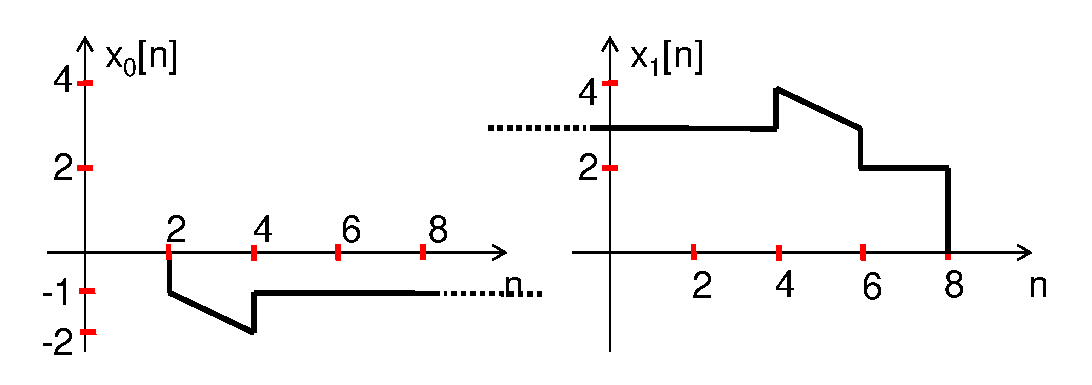
\includegraphics[width=.9\textwidth]{fig1.eps}
\end{figure}





\vspace{1cm}

\noindent \textbf{4.} (7 points) Consider the following interconnection of LTI systems:

\begin{figure}[h!]
\centering
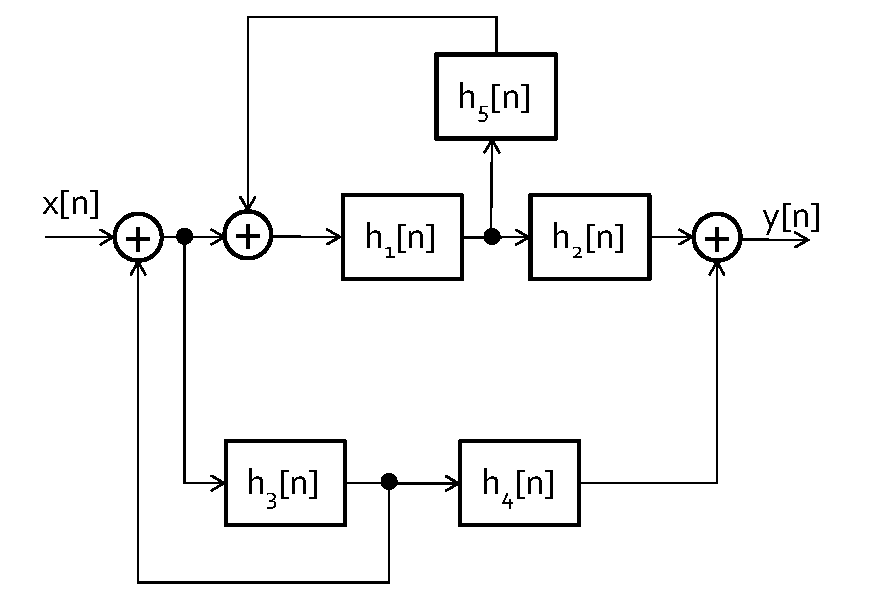
\includegraphics[width=.8\textwidth]{fig2.eps}
\end{figure}

Express the frequency response of the overall system $H(e^{j\omega})$ in terms of the frequency responses of the subsystems depicted in the diagram. Assume that $h_3[n]=\delta[n-1]$. Would the overall system be stable in general? If not, find an example of bounded input sequence $x[n]$ that would make the system unstable (i.e. the output sequence $y[n]$ would be unbounded). 


\end{document}